\documentclass[aps,pra,twocolumn,superscriptaddress,floatfix,nofootinbib]{revtex4-2}

\usepackage{amsmath}
\usepackage{amssymb}
\usepackage{graphicx}
\usepackage[colorlinks=true,linkcolor=blue,citecolor=blue,urlcolor=blue]{hyperref}

\begin{document}

\title{A uniform memory cutoff is optimal in a swap-asap repeater chain, and an
       accumulated-decay gate is dominated rather than trading}

\author{Faruk Sami Bilgin}
\email{fsamibilgin@gmail.com}
\affiliation{Independent researcher}

\date{\today}

\begin{abstract}
Two enrichments of the simplest repeater memory cutoff have been reported as
making no measurable difference: indexing the cutoff by the span of the stored
link, and replacing the age gate by a threshold on accumulated decoherence. We
re-measure both with policies driven by shared randomness --- each elementary
link owns a geometric stream, and its $k$-th generation consumes that stream's
$k$-th variate whichever policy asked --- a coupling that survives a stricter
policy consuming more draws, which a shared generator does not. Two
methodological points decide the outcome, and both cut against our own earlier
version of this measurement. First, a span exponent $\gamma$ must be compared
with the cutoff \emph{scale} re-optimised at each $\gamma$: holding $c_0$ at its
$\gamma=0$ optimum, as is natural and as we did, confounds the exponent with the
scale and manufactures a large asymmetry that is not there. Re-tuned, a uniform
cutoff is optimal at both geometries studied and the penalty for departing from
it is small and nearly symmetric --- $0.5$--$1.3\%$ at $|\gamma|=0.25$, rising
to $6$--$20\%$ at $|\gamma|=1$. Second, two policies must be compared at matched
delivery time, not at their separately tuned operating points: a slower policy
delivering a better state is the definition of a trade-off, not evidence of one.
On the matched comparison the accumulated-decay gate is not trading. At $4$
segments it coincides with the age gate to within $0.02\%$ in delivered Werner
parameter; at $8$ segments it is \emph{dominated on both axes}, delivering a
worse state ($0.8289$ against $0.8364$) in less time and losing $10.4\%$ of the
key rate. We also close the validation gap, checking the generation layer
against Praxmeyer's exact $N$-segment with-cutoff expression at $22$ parameter
points and against the Khatri \emph{et al.} bracket.
\end{abstract}

\maketitle

\section{Introduction}

Entanglement stored in a repeater memory decoheres, so a link that waits too
long for its partner is worth discarding and remaking. The resulting cutoff
policy is not optional, and the key rate is non-monotone in the
cutoff~\cite{Collins2007,Rozpedek2018,Khatri2019,Li2021}.

Whether a \emph{richer} policy helps is less settled. The cutoff can be indexed
by how much of the chain a stored link already spans,
$t_{\rm cut}({\rm span}) = c_0\,{\rm span}^{\gamma}$, since discarding a long
link throws away more work. Or the age gate can be replaced by a gate on the
accumulated decoherence --- discard when the Werner parameter falls below
$w_{\min}$ --- which is closer to the quantity that matters. The level-indexed
version of the first has been proposed and optimised~\cite{Santra2019} and
measured against a uniform baseline in a nested protocol~\cite{Li2021} with no
significant gain, restated independently~\cite{Reiss2023}.

Our own earlier runs in a parallel swap-asap chain measured the span-indexed
family at $-2.07\%$ against a two-sigma band of $\pm1.9\%$ --- outside the band,
and so a difference rather than a null --- and the accumulated-decay gate at
$-0.41\%$ against $\pm1.7\%$, which was a null at that resolution and excluded
nothing tighter than a $1.7\%$ gap. This paper tightens both, and in doing so
overturns two things we previously reported.

\section{Method}

\subsection{Coupling by source}

Almost all the variance is shared: the policies run the same chain, the same
link generation, the same decoherence, and differ only in when a stored link is
discarded. The obvious coupling --- one seeded generator per replicate, reused
across policies --- fails here, and the reason is generic to policy comparison
in queueing-like models. A stricter cutoff triggers more rebuilds, so the
policies consume \emph{different numbers} of variates; a shared generator
desynchronises at the first divergent rebuild, which is exactly where the
policies begin to differ.

We couple by source instead. Every elementary link $j$ owns a stream, and the
$k$-th generation attempt on link $j$ draws the $k$-th variate of stream $j$
regardless of which policy asked, when, or how many draws other links consumed.
When a merged link spanning $[\,j, j+s)$ is rebuilt, its $s$ constituents each
draw from their own streams and the rebuild takes the maximum. The engine
reproduces the original in distribution: mean delivery time $0.1856$~s against
$0.1873$~s ($0.89\sigma$), mean Werner parameter to $0.01\%$.

The gain is real but modest, and worth stating precisely rather than
rhetorically. Against the unpaired comparison the standard error on the
difference falls $2.4\times$; at matched sample count the coupling itself
contributes $1.34\times$ and the rest is a $3.3\times$ larger ensemble. The
limit is the Werner channel, where the pair correlation is only $0.145$ and
$0.043$ at the two geometries, against $0.13$--$0.81$ for the delivery time. The
figure of merit is $r(\bar w)/\bar T$ with $r$ the BB84 fraction --- a function
of the \emph{mean} Werner parameter, which is why the pairing buys less than the
delivery-time correlations suggest.

\subsection{Two comparisons that have to be set up correctly}

\paragraph*{The exponent must be separated from the scale.} Since
$t_{\rm cut} = c_0\,{\rm span}^{\gamma}$, changing $\gamma$ at fixed $c_0$
changes the cutoff's overall magnitude as well as its span dependence: at $8$
segments, $\gamma=+1$ hands a span-$8$ link $320$ slots while $\gamma=-1$ hands
it $5$. A landscape swept at fixed $c_0$ is therefore mostly the scale being
wrong. We re-tune $c_0$ over a $16$-point grid at every $\gamma$, so each point
is that exponent's best achievable policy. Our previous version did not, and
Sec.~\ref{sec:gamma} reports what that cost.

\paragraph*{Policies must be compared at matched delivery time.} Two policies
tuned separately land at different operating points, and a slower one delivering
a better state is the shape of any rate--fidelity trade-off, not evidence that
the policies differ. The question is whether the two families trace different
\emph{frontiers}, which requires both swept.

\subsection{A cap, and what it is for}

One corner of the tuning grid does not merely perform badly but fails to
progress: a link's lifetime under the accumulated-decay gate is
$(T_{\rm coh}/\Delta t)\log(w_{\rm now}/w_{\min})$, so as $w_{\min}$ approaches
the Werner parameter of a fresh link the lifetime goes to zero and the link is
discarded about as fast as it is built. At $8$ segments with $w_{\rm init}=0.99$
the grid point $w_{\min}=0.95$ leaves roughly a fifth of samples undelivered at
a cap of $400\times$ the no-cutoff mean. We cap a delivery there and report the
censored fraction with every number. No result below rests on a censored point:
every censored fraction in the reported runs is exactly zero.

\section{The span exponent}
\label{sec:gamma}

\begin{figure}[t]
  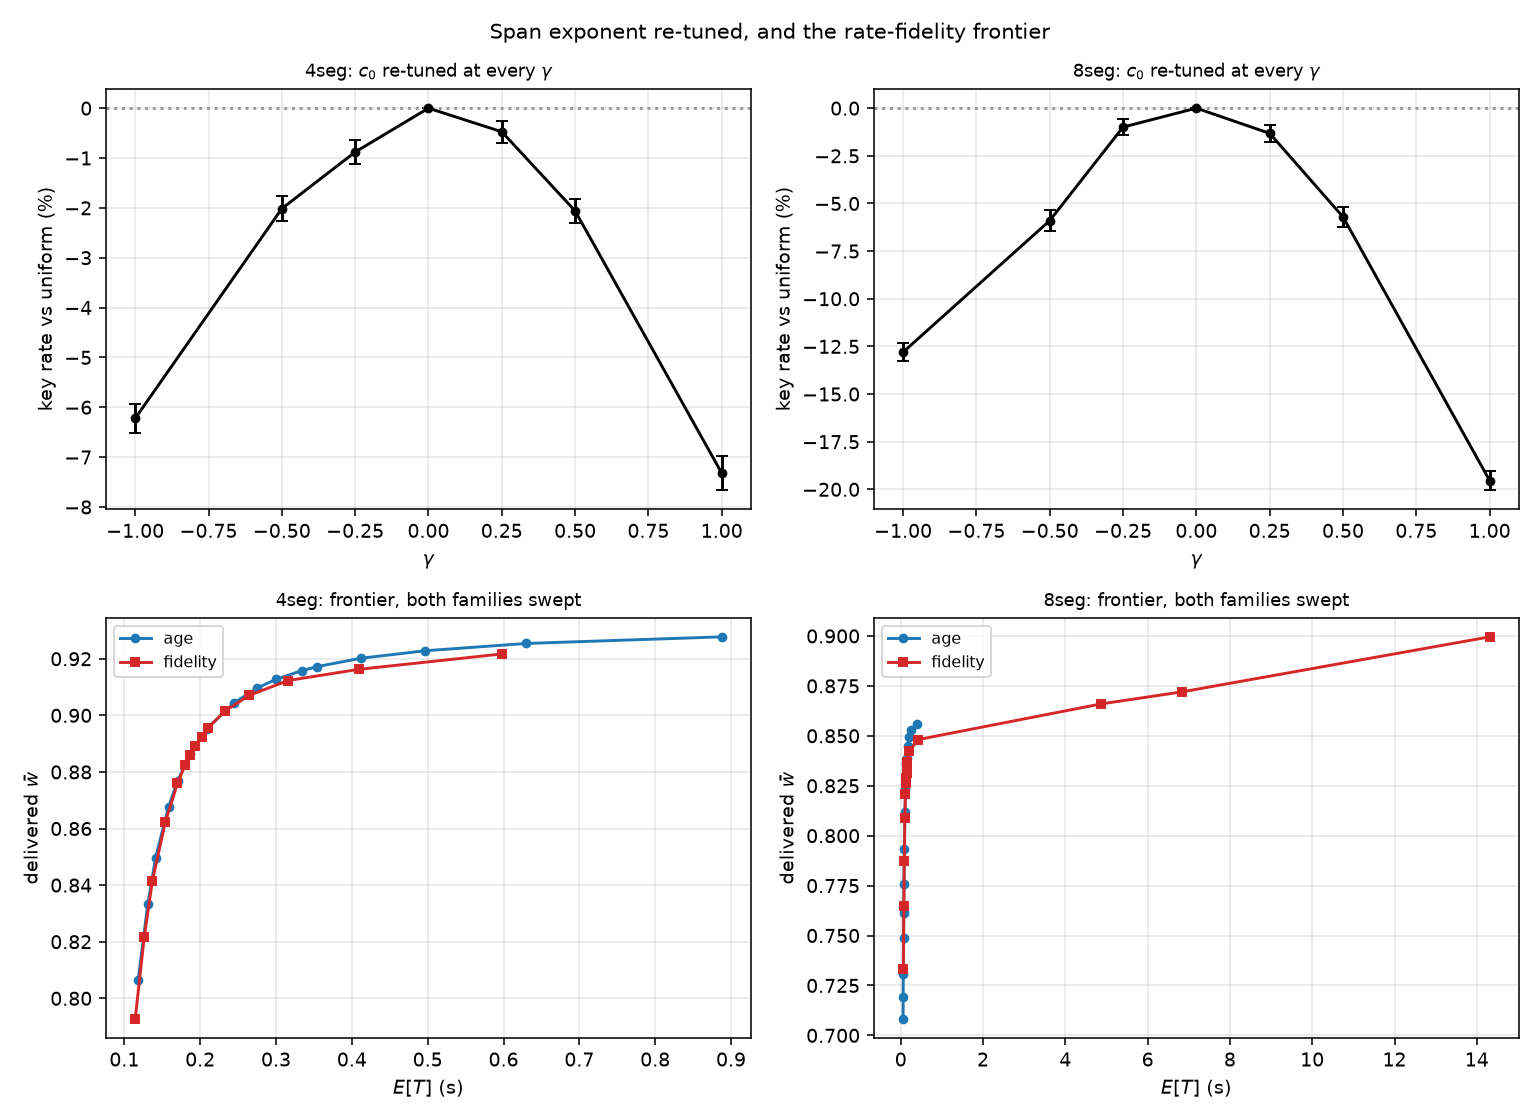
\includegraphics[width=\columnwidth]{figs/retuned_landscape.png}
  \caption{Top: key rate against a uniform cutoff as a function of the span
  exponent, with $c_0$ re-optimised at every $\gamma$. Bottom: the
  rate--fidelity frontier with both families swept. Error bars are paired
  block-jackknife standard errors.}
  \label{fig:retuned}
\end{figure}

\begin{table}[b]
  \caption{Paired difference in secret-key rate against a uniform cutoff, with
  $c_0$ re-tuned at each $\gamma$. $c_0^\star$ is the tuned scale; its
  systematic drift with $\gamma$ is what a fixed-$c_0$ sweep confounds with the
  exponent.}
  \label{tab:gamma}
  \begin{ruledtabular}
  \begin{tabular}{lcccc}
    & \multicolumn{2}{c}{4 seg, 400 km} & \multicolumn{2}{c}{8 seg, 600 km}\\
    $\gamma$ & $c_0^\star$ (s) & $\Delta$ & $c_0^\star$ (s) & $\Delta$\\
    \colrule
    $-1.00$ & 0.050 & $-6.22\%$ & 0.035 & $-12.80\%$ \\
    $-0.50$ & 0.040 & $-2.02\%$ & 0.025 & $-5.90\%$ \\
    $-0.25$ & 0.035 & $-0.88\%$ & 0.017 & $-0.99\%$ \\
    $0$     & 0.030 & ---       & 0.012 & --- \\
    $+0.25$ & 0.025 & $-0.47\%$ & 0.010 & $-1.32\%$ \\
    $+0.50$ & 0.025 & $-2.06\%$ & 0.008 & $-5.71\%$ \\
    $+1.00$ & 0.015 & $-7.32\%$ & 0.004 & $-19.54\%$ \\
  \end{tabular}
  \end{ruledtabular}
\end{table}

Table~\ref{tab:gamma} is the landscape with the scale re-optimised. A uniform
cutoff is optimal at both geometries --- which confirms the established
conclusion --- and the penalty for departing is small and nearly symmetric:
$0.47$--$1.32\%$ at $|\gamma|=0.25$ (resolved at $2.1$--$3.7\sigma$),
$2.0$--$5.9\%$ at $|\gamma|=0.5$, and $6$--$20\%$ at $|\gamma|=1$. The residual
asymmetry at $8$ segments, $-12.80\%$ against $-19.54\%$ at $\gamma=\mp1$, is
the only sign of one.

This replaces a much stronger claim we made from the same data swept at fixed
$c_0$, where the same points read $-38.02\%$ and $-100\%$ and the
$\gamma=+0.25$ point read $-22.99\%$ at $36\sigma$. That point is
$-1.32\%$ at $2.9\sigma$ once the scale is re-optimised. We had concluded that
``granting longer cutoffs to longer-span links is the direction that fails, and
it fails harder as the chain grows''; the tuned $c_0^\star$ column shows why
that was an artifact --- the optimal scale falls monotonically with $\gamma$, by
$3.3\times$ at $4$ segments and $8.75\times$ at $8$, so a fixed-$c_0$ sweep
moves progressively further from the optimum in both directions and further at
the larger geometry.

\section{The accumulated-decay gate}

\begin{table}[b]
  \caption{Matched-delivery-time comparison. The age policy listed is the one
  whose mean delivery time is closest to the tuned fidelity gate's.}
  \label{tab:matched}
  \begin{ruledtabular}
  \begin{tabular}{llccc}
    & policy & $E[T]$ (s) & $\bar w$ & key (Hz)\\
    \colrule
    4 seg & age, $c_0=0.030$        & 0.1865 & 0.8862 & 1.98398\\
          & fidelity, $w_{\min}=0.895$ & 0.1871 & 0.8860 & 1.97385\\
    \colrule
    8 seg & age, $c_0=0.013$        & 0.1390 & 0.8364 & 1.31668\\
          & fidelity, $w_{\min}=0.895$ & 0.1326 & 0.8289 & 1.18427\\
  \end{tabular}
  \end{ruledtabular}
\end{table}

At $4$ segments the two families coincide. At matched delivery time
(Table~\ref{tab:matched}) they agree to $0.02\%$ in delivered Werner parameter
and $0.5\%$ in key rate; the frontiers lie on top of each other. That, rather
than a difference inside an error bar, is the content of the $4$-segment null,
and it is a stronger statement than the one we made before: the earlier
$+0.01\pm0.35\%$ excluded a gap above $0.7\%$, where the unpaired comparison
excluded $1.7\%$ --- a $2.45$-fold tightening, not the seventeen-fold we
previously claimed, which came from transcribing Ref.~\cite{Li2021}'s measured
policy gap as though it were our own error bar.

At $8$ segments they do not coincide, and the difference is not a trade. The
fidelity gate delivers a \emph{worse} state ($0.8289$ against $0.8364$) in
\emph{less} time, and loses $10.4\%$ of the key rate against the best age policy
($1.18427$ against $1.32199$~Hz). It is dominated on both axes. Our previous
explanation --- that the gate buys state quality with time and the time cost
compounds down the chain --- was read off two separately tuned operating points
and has the sign backwards.

A mechanism consistent with the data, offered as such and not as a
demonstration: an absolute floor on $w$ imposes wildly different holding times
by span. At $w_{\min}=0.90$ and $T_{\rm coh}=0.5$~s the implied maximum hold is
$47.7$, $37.6$, $27.6$, $17.5$, $7.5$, $0$, $0$~ms for spans $1$ through $7$ ---
an effective $\gamma\simeq-1$, with spans $6$ and $7$ discarded at the instant
of creation because $0.99^{11} = 0.8953 < w_{\min}$. At $4$ segments the largest
gated span is $3$ and $0.99^{5} = 0.9510 > w_{\min}$, so this cannot occur, and
the effective exponent is $\simeq-0.45$. Table~\ref{tab:gamma} independently
penalises strongly negative $\gamma$ at $8$ segments and barely at $4$. We note
one test against this reading: exempting the born-dead spans makes the gap
\emph{worse}, so their existence is a real pathology of the tuned policy but is
not the proximate cause.

\section{Validation in the with-cutoff regime}

Our only analytic check had been a two-segment, no-cutoff identity, while every
result lives in the with-cutoff regime.

Praxmeyer~\cite{Praxmeyer2013} gives the expected number of slots for $N$
segments under a global cutoff --- all $N$ links up within $\tau$ slots of the
first success, or the round restarts --- in closed form. We reproduce both
limits she proves, $\tau=0\to p^{-N}$ and
$\tau\to\infty\to\sum_k(-1)^{k+1}\binom{N}{k}/(1-q^k)$, to $10^{-13}$, then
compare against a vectorised simulation of her rule at $N\in\{2,4,8\}$,
$p\in\{0.1,0.3\}$, $\tau\in\{1,3,10,30\}$. The worst deviation is $2.85\sigma$
over $22$ simulated points, with two points formula-only because their expected
round exceeds the slot budget. For $22$ independent normals the expected maximum
$|z|$ is $2.20$ and the observed value sits at the $91$st percentile, with
$\chi^2 = 22.9$ on $22$ degrees of freedom: a pass. Her rule is an end-to-end
restart rather than our per-link discard, so this validates the generation layer
and the slot accounting under a different policy, which is where an off-by-one
would live.

The bracket of Khatri \emph{et al.}~\cite{Khatri2019} holds at every cutoff we
sweep to within two standard errors. Eight of $27$ sweep points sit below the
exact lower bound by at most $1.4\sigma$; the lower bound is the
$\tau\to\infty$ limit that the sweep approaches from above, so this is the
expected behaviour of a Monte Carlo estimate near a bound it approaches, not a
violation. The upper bound $p^{-M}$ is $10^{8}$ at $M=8$, $p=0.1$ against
observations of $26$--$188$, and is vacuous there.

\section{Limitations}

One protocol, one decoherence model, two geometries, one figure of merit. The
$4$-versus-$8$ comparison changes segment count, total length, segment length,
generation probability and slot duration together; a control separating them
shows segment count is the driver and length pushes the other way (at fixed
$400$~km, $4\to8$ segments moves the gap from $-0.2\%$ to $-16.2\%$; at fixed
$4$ segments, $400\to600$~km moves it to $+3.6\%$, where the fidelity gate
wins). ``Compounds down the chain'' is still asserted from two segment counts.

One model detail matters for a paper about span dependence: on expiry the
rebuilt link is credited $w_{\rm init}^{s}w_{\rm swap}^{s-1}$ with no
decoherence during the rebuild wait, so the constituents that finish early
accrue none. For $s=6$ at $8$ segments the skipped wait averages about
$0.06\,T_{\rm coh}$, which is an order of magnitude larger than the fidelity
differences in Table~\ref{tab:matched}. It is common-mode in a paired
difference, but it is span-dependent, and we have not measured the residual.

Finally, the span-indexed family is one parametrisation of one axis, and the
result that its optimum sits at $\gamma=0$ is a statement about this protocol;
in a nested doubling protocol the level axis is the natural one and has its own
literature~\cite{Santra2019,Li2021}.

\begin{thebibliography}{9}

\bibitem{Collins2007}
  O.~A.~Collins, S.~D.~Jenkins, A.~Kuzmich, and T.~A.~B.~Kennedy,
  Phys.\ Rev.\ Lett.\ \textbf{98}, 060502 (2007).

\bibitem{Rozpedek2018}
  F.~Rozp\k{e}dek \emph{et al.},
  Phys.\ Rev.\ A \textbf{97}, 062333 (2018).

\bibitem{Khatri2019}
  S.~Khatri, C.~T.~Matyas, A.~U.~Siddiqui, and J.~P.~Dowling,
  Phys.\ Rev.\ Research \textbf{1}, 023032 (2019).

\bibitem{Li2021}
  B.~Li, T.~Coopmans, and D.~Elkouss,
  IEEE Trans.\ Quantum Eng.\ \textbf{2}, 4103015 (2021).

\bibitem{Santra2019}
  S.~Santra, L.~Jiang, and V.~S.~Malinovsky,
  Quantum Sci.\ Technol.\ \textbf{4}, 025010 (2019).

\bibitem{Reiss2023}
  F.~Reiss and P.~van~Loock,
  Phys.\ Rev.\ A \textbf{108}, 032417 (2023).

\bibitem{Praxmeyer2013}
  L.~Praxmeyer,
  \emph{Reposition time in probabilistic imperfect memories},
  \href{https://arxiv.org/abs/1309.3407}{arXiv:1309.3407} (2013).

\end{thebibliography}

\end{document}
